\chapter{O Prazo}

\begin{center}
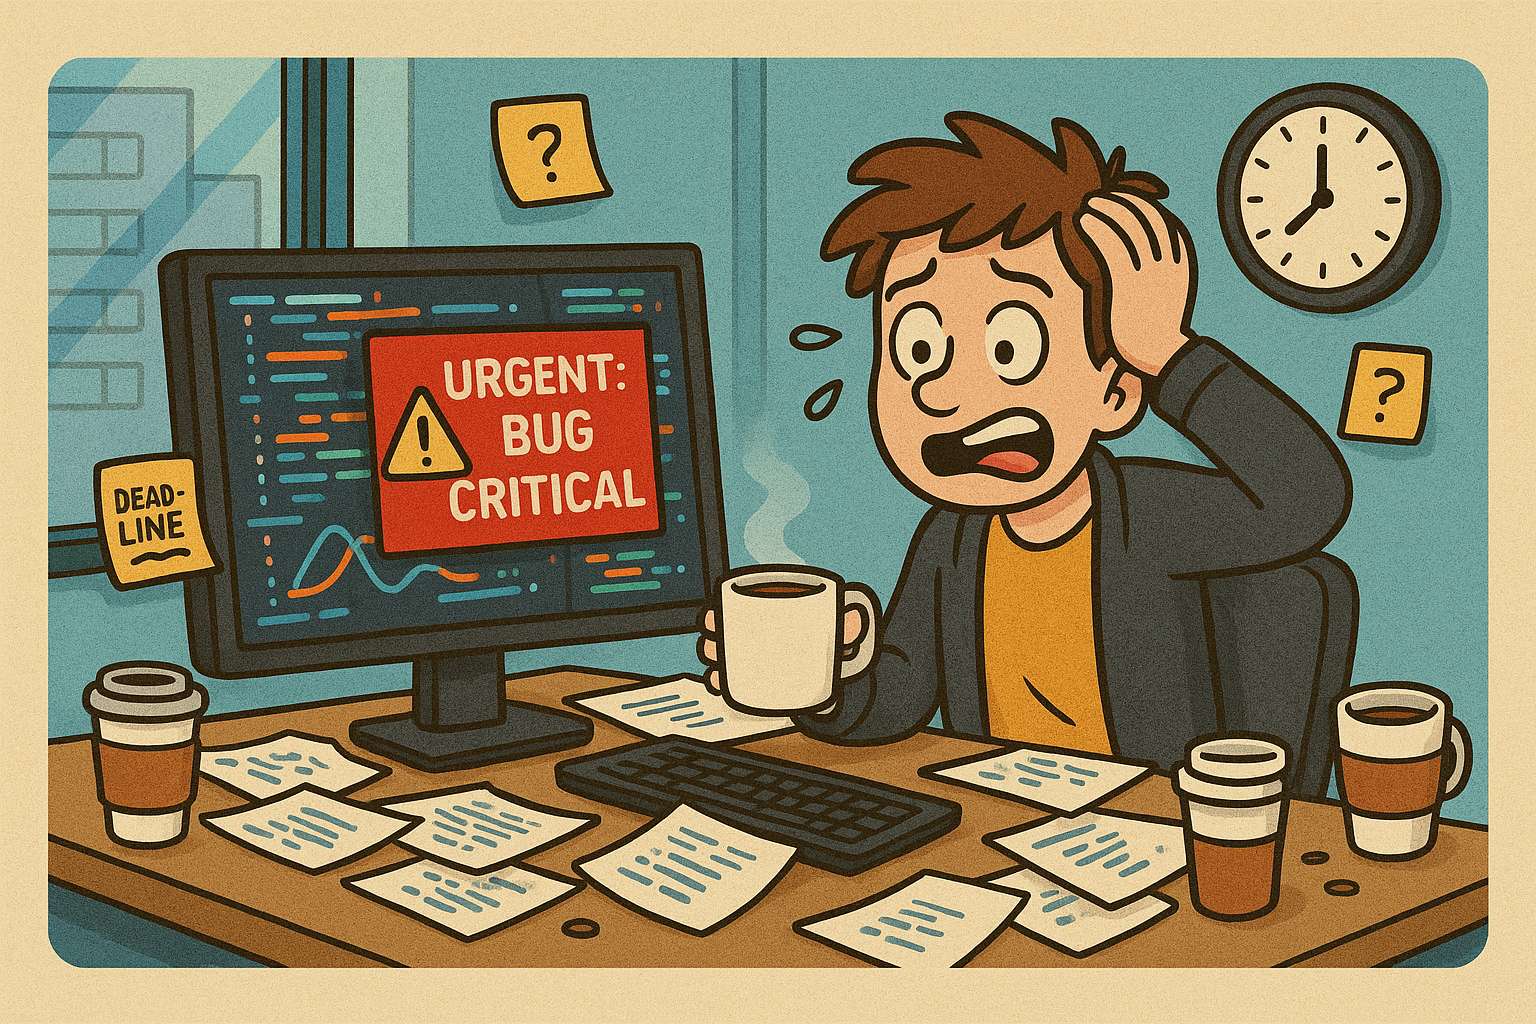
\includegraphics[width=0.5\linewidth]{Images/prazo.png}    
\end{center}
\vspace{0.5cm}

Como todo projeto, uma dissertação ou tese tem que ter um fim. Um limitante importantíssimo para isso é o prazo que a instituição dá para o aluno completar o seu processo.

Você deve tentar atingir não os prazos máximos da instituição, que podem ser mais flexíveis, mas sim os prazos das bolsas dadas pela CAPES e CNPq: mestrado 2 anos, doutorado 4 anos.

Sabemos que esses prazos são pequenos e eu sugiro que no máximo se chegue a 2,5 anos e 4,5 anos.

Gravidez recebe um prazo adicional, por lei. Doenças graves costumam obter prazos adicionais, por meio de processos institucionais\footnote{Um aluno meu que teve AVC dias antes de sua defesa, e ficou um bom tempo sem memória de longo prazo, foi totalmente atendido com todo o prazo que precisou para se encontrar em plenas condições de defender a dissertação. Felizmente, ele se recuperou e foi aprovado na defesa.}.

\needspace{5\baselineskip}
\section{De trás para frente}

Seja o prazo institucional, o das bolsas, ou o que você deu a si mesmo, é importante fazer a ``conta de trás para frente'' para saber não só quando deve alcançar seus objetivos, mas também quando deve realizar os atos burocráticos que permitem você defender a tese.

Para isso, a construção de um cronograma é fator de apoio. Para mim, cronogramas são obras de ficção, pois são o desejável, mas raramente o real. O problema é que se você não tem um plano, não sabe para onde ir, se está atrasada ou adiantada (o que é muito raro), e não pode fazer um replanejamento. Nas qualificações é importante colocar um plano de trabalho na forma de cronograma.

\CoppeWay{Os prazos da Coppe e da UFRJ}{
O exame de \textbf{seminário de mestrado} tem prazo de \textbf{dois anos sem extensão possível}.

A Coppe limita o prazo de uma \textbf{dissertação em 3 anos}, mais meio ano de uma possível extensão que, pelo regulamento, não será dada facilmente.

O limite de uma \textbf{tese é de 5 anos}, com possível \textbf{extensão} (que novamente provavelmente não será dada) \textbf{de 1 ano}, com \textbf{o exame de qualificação tendo prazo de 3 anos, com uma extensão de seis meses possível}.

Atualmente é possível trancar a matrícula por até dois períodos na Coppe, sem contar prazo\footnote{Essa mudança é recente, antes o prazo contava, só não era obrigado a fazer cadeiras.}.
}


\section{O que acontece se você usa o prazo máximo?}

Vamos esquecer, momentaneamente, que você pode PERDER O PRAZO, sendo reprovado pelo prazo, o que é perder o trabalho de anos. Quais os outros problemas?

Primeiro, o texto sai muito pior do que devia, os experimentos são terminados de forma açodada. A banca vai reclamar muito e provavelmente reprovar com restrições e te dar um dever de casa.

Segundo, a capacidade do orientador ajudar em algo nesses casos (fim do seu prazo) é muito reduzida. Por quê? Porque seu orientador tem outras coisas para fazer no trabalho e uma vida pessoal\footnote{Aconteceu comigo, tive uma doença grave junto com o prazo final de muito alunos, incluindo 6 meses de licença, 50  dias de hospital e uma cirurgia de coração aberto. Conseguimos resolver o problema de todos, mas não foi uma boa experiência para ninguém. Mais tarde, tive Covid, fui entubado e fiquei meses sem trabalhar novamente.}, que inclui outros orientados provavelmente também fazendo a mesma coisa.
Isso significa que o orientador, não vai poder realmente orientar o seu final de tese, o que é muito ruim, mas é o que acontece na prática.

Não é razoável você esperar que depois de ficar 5(3) anos fazendo seu trabalho sem muito interesse, no último instante queira uma dedicação emergencial do seu orientador. 
Ele estava lá por muito tempo. Pode ser que, algumas vezes, ele consiga essa dedicação, mas também pode ser que não.

Ou seja, o seu risco, como orientado, aluno e candidato ao título cresce quando o prazo está chegando. Cuidado!

\section{O Que Acontece Se Você Não Defender?}

Para algumas pessoas, desistir da tese é um alívio. Isso porque pode ser muito difícil manter a tese sendo trabalhada e o resto da vida funcionando. Não só fatos negativos, como parentes doentes e problemas no emprego, mas também fatos positivos, como novas perspectivas de vida e oportunidades imperdíveis.

Se por algum motivo você não defende a tese, a verdade é que, para a instituição, não há um problema real. Há uma baixa nas notas de avaliação, mas provavelmente muito pequena, já que tudo é planejado para haver algumas perdas na média.

Porém, se você ganhou uma bolsa, tudo muda, porque você será cobrado para devolver a bolsa. Então será necessária uma justificativa, como um problema que teve que resolver, ou simplesmente aceitar o fato que você seguiu por outro caminho e é melhor pagar de uma vez. Porém, não ache que a bolsa é um presente, ela exige uma contrapartida, que é a defesa da tese. Apesar de a bolsa ser pequena, o valor a ser devolvido será alto, pois inclui todos os valores recebidos mais a correção financeira.






